%%%%%%%%%%%%%%%%%%%%%%%%%%%%%%%%%%%%%
%                                   %
% Compile with XeLaTeX and biber    %
%                                   %
% Questions or comments:            %
%                                   %
% joshua dot mcneill at uga dot edu %
%                                   %
%%%%%%%%%%%%%%%%%%%%%%%%%%%%%%%%%%%%%

\documentclass{beamer}
  % Read in standard preamble (cosmetic stuff)
  %%%%%%%%%%%%%%%%%%%%%%%%%%%%%%%%%%%%%%%%%%%%%%%%%%%%%%%%%%%%%%%%
% This is a standard preamble used in for all slide documents. %
% It basically contains cosmetic settings.                     %
%                                                              %
% Joshua McNeill                                               %
% joshua dot mcneill at uga dot edu                            %
%%%%%%%%%%%%%%%%%%%%%%%%%%%%%%%%%%%%%%%%%%%%%%%%%%%%%%%%%%%%%%%%

% Beamer settings
% \usetheme{Berkeley}
\usetheme{CambridgeUS}
% \usecolortheme{dove}
% \usecolortheme{rose}
\usecolortheme{seagull}
\usefonttheme{professionalfonts}
\usefonttheme{serif}
\setbeamertemplate{bibliography item}{}

% Packages and settings
\usepackage{fontspec}
  \setmainfont{Charis SIL}
\usepackage{hyperref}
  \hypersetup{colorlinks=true,
              allcolors=blue}
\usepackage{graphicx}
  \graphicspath{{../../figures/}}
\usepackage[normalem]{ulem}
\usepackage{enumerate}

% Document information
\author{M. McNeill}
\title[FREN2001]{Français 2001}
\institute{\url{joshua.mcneill@uga.edu}}
\date{}

%% Custom commands
% Lexical items
\newcommand{\lexi}[1]{\textit{#1}}
% Gloss
\newcommand{\gloss}[1]{`#1'}
\newcommand{\tinygloss}[1]{{\tiny`#1'}}
% Orthographic representations
\newcommand{\orth}[1]{$\langle$#1$\rangle$}
% Utterances (pragmatics)
\newcommand{\uttr}[1]{`#1'}
% Sentences (pragmatics)
\newcommand{\sent}[1]{\textit{#1}}
% Base dir for definitions
\newcommand{\defs}{../definitions}


  % Packages and settings

  % Document information
  \subtitle[Sites et \lexi{où} et \lexi{qui}]{Les sites et les relatifs \lexi{où} et \lexi{qui}}

\begin{document}
  % Read in the standard intro slides (title page and table of contents)
  \begin{frame}
    \titlepage
    \tiny{Office: % Basically a variable for office hours location
Gilbert 121\\
          Office hours: % Basically a variable for office hours
 lundi, mercredi, vendredi 10:10--11:10
}
  \end{frame}

  \begin{frame}[t]{Décrivons-les}
    \begin{columns}
      \column{0.5\textwidth}
        Décrivons les endroits suivants en utilisant des pronoms relatifs.
        \begin{enumerate}
          \item C'est une cave où/qui ...
          \item<2-> C'est un village médiéval où/qui ...
          \item<3-> C'est une abbaye où/qui ...
          \item<4-> C'est un théâtre romain où/qui ...
          \item<5-> C'est une cuisine où/qui ...
        \end{enumerate}
      \column{0.5\textwidth}
        \begin{minipage}[c][0.8\textheight]{\linewidth}
          \begin{center}
            \only<1>{
              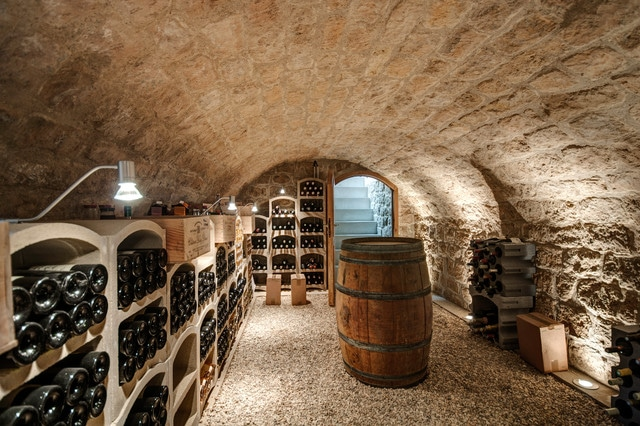
\includegraphics[scale=0.25]{cave.jpg}
            }
            \only<2>{
              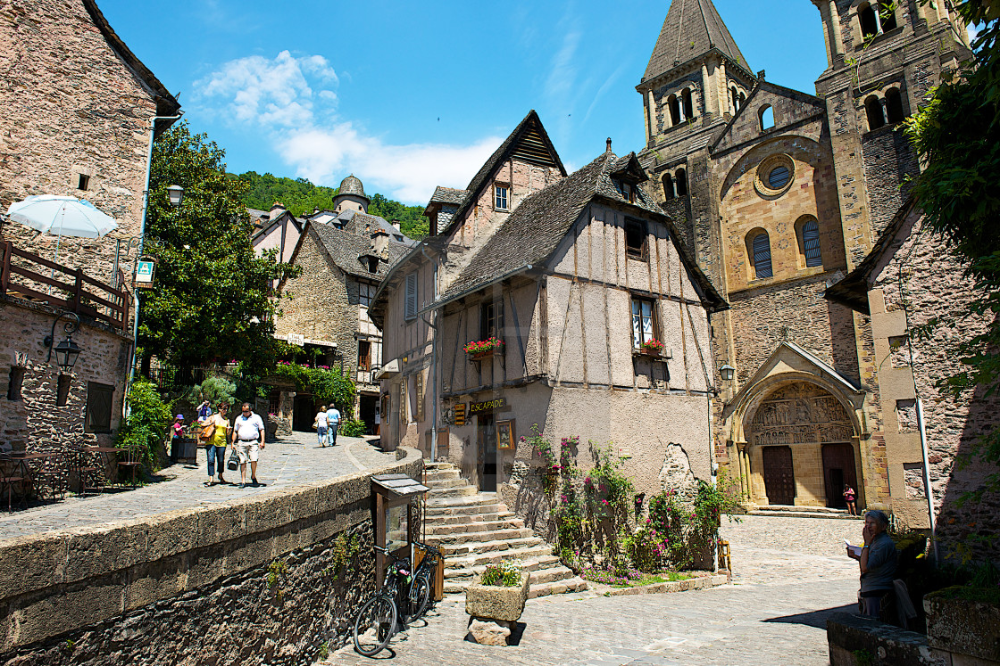
\includegraphics[scale=0.16]{village_médiéval.png} \\
              Conques, France
            }
            \only<3>{
              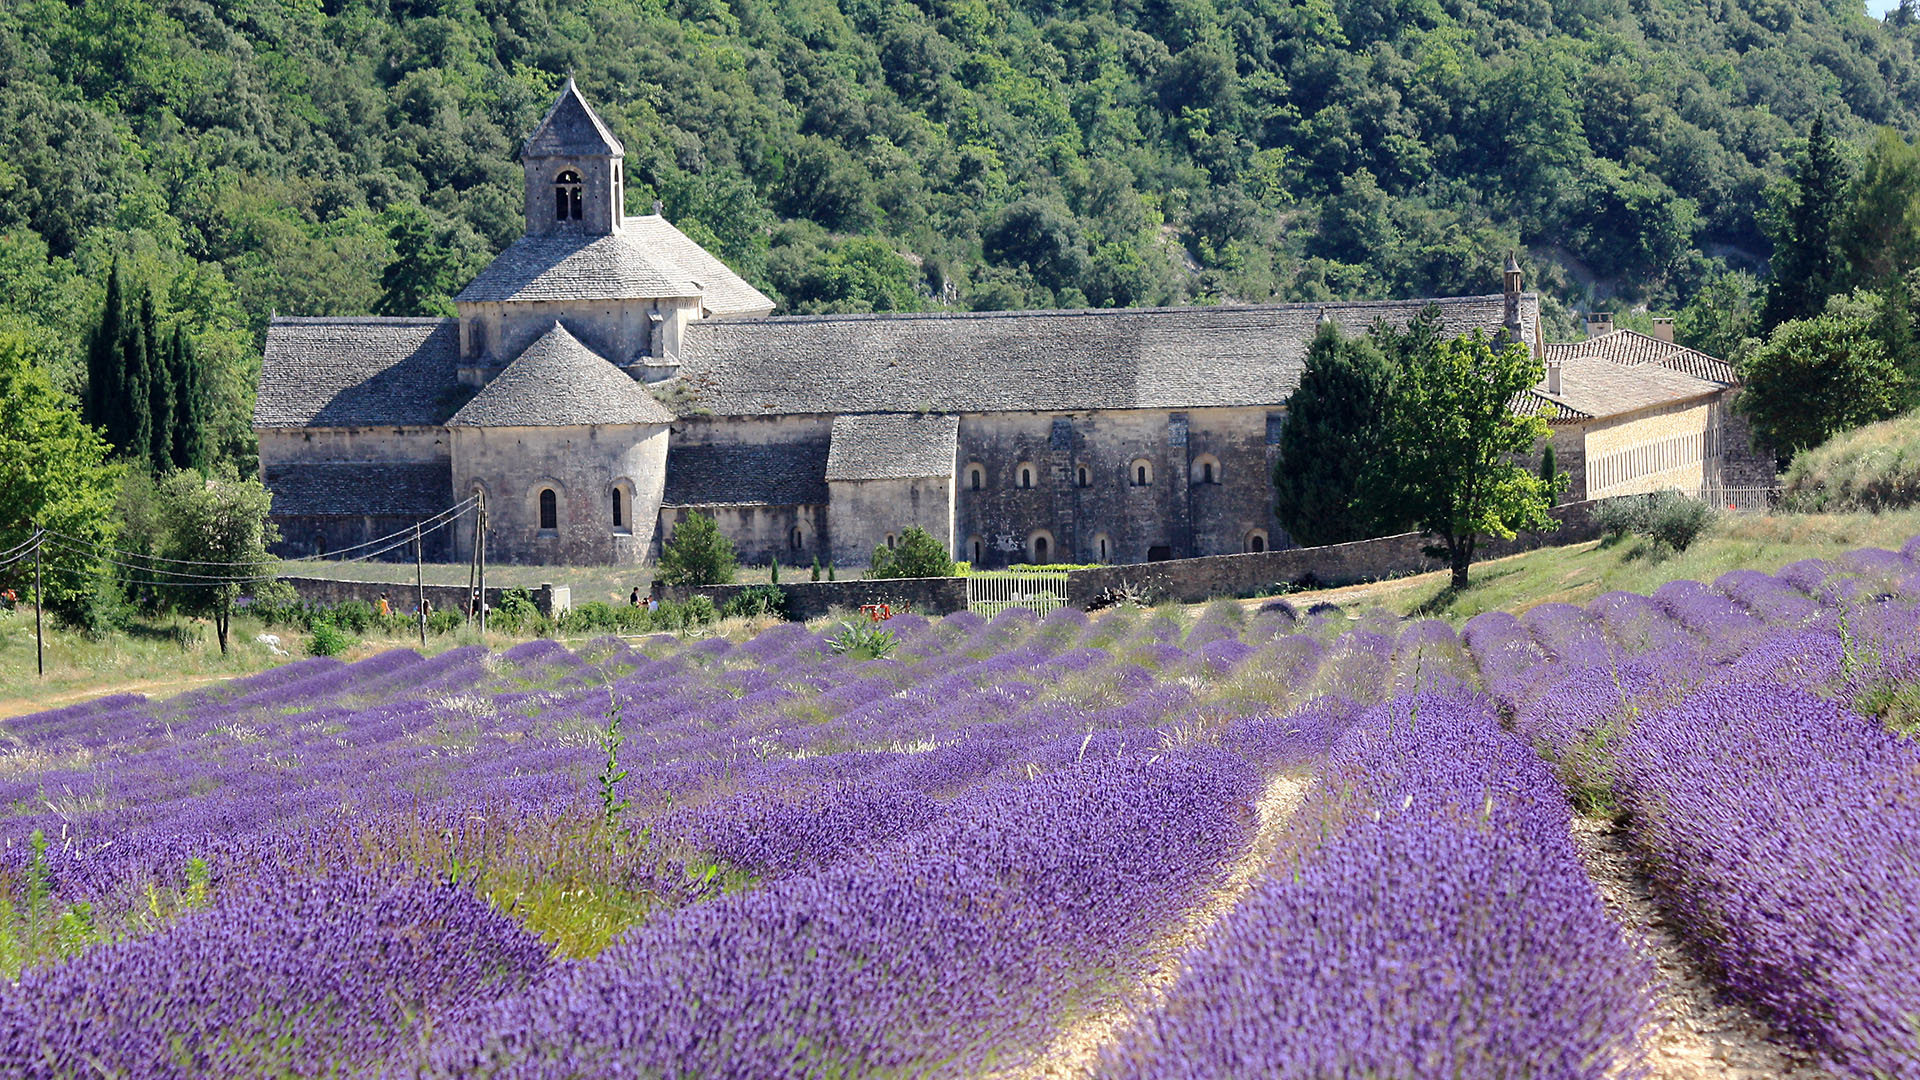
\includegraphics[scale=0.22]{abbaye.jpg} \\
              L'abbaye Notre-Dame de Sénanque
            }
            \only<4>{
              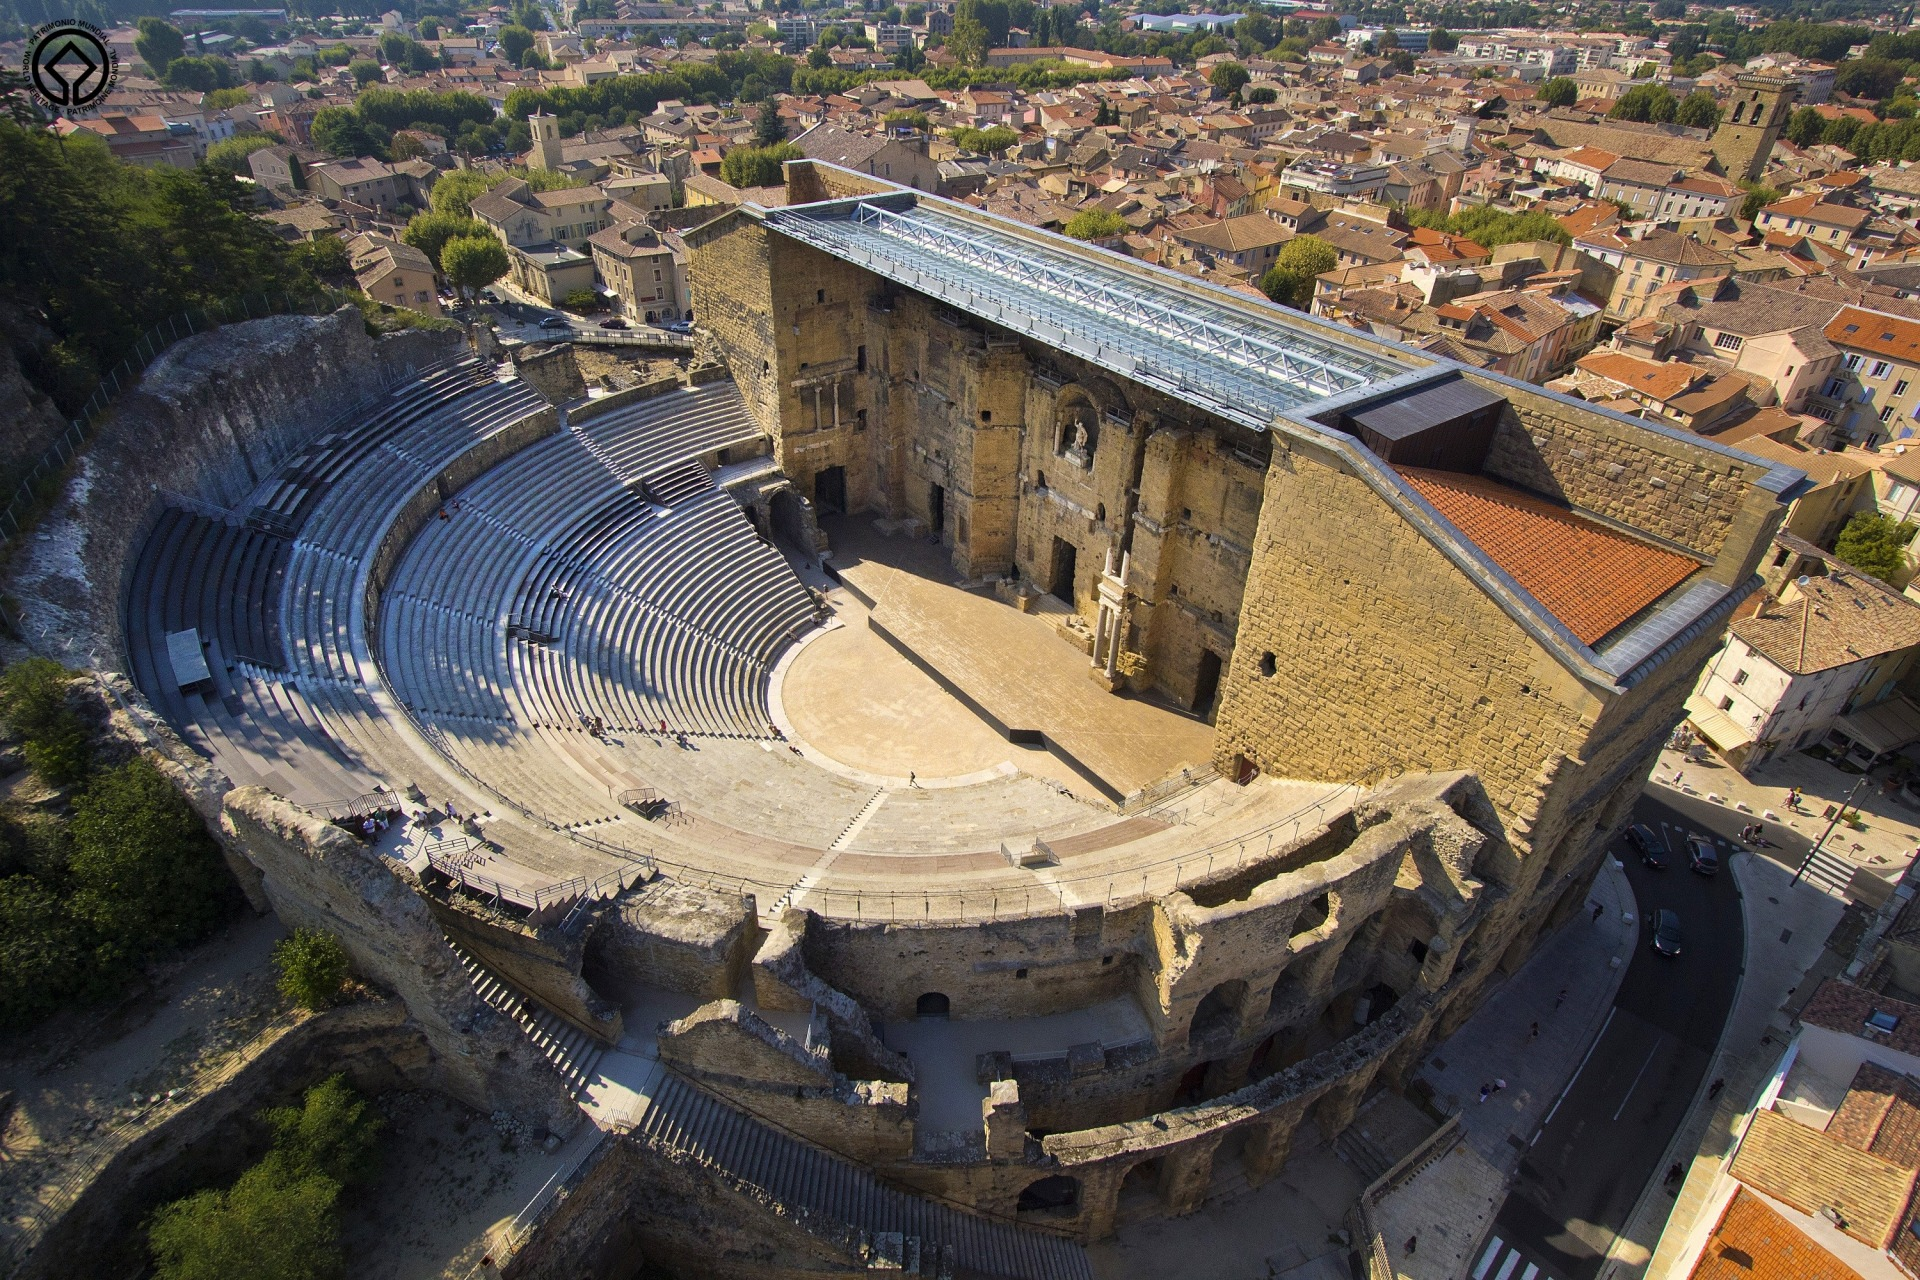
\includegraphics[scale=0.11]{théâtre_romain.jpg}
              Théâtre antique d'Orange
            }
            \only<5>{
              
\includegraphics[scale=0.25]{cuisine.jpg}
            }
          \end{center}
        \end{minipage}
    \end{columns}
  \end{frame}

  \begin{frame}{}
    \begin{center}
      \Large Quiz
    \end{center}
  \end{frame}

  \begin{frame}{En quelles saisons?}
    \small
    Avec un/e partenaire, discutez en quelles saisons tu \alert{aimes}, \alert{as envie de} ou \alert{préfères} faire les activités suivantes, et pourquoi.
    \begin{description}
      \item[] \textbf{Modèle:} \textit{voyager dans les pays tropicaux}
      \item[E1:] L'hiver est la saison \textcolor{red}{où} \alert{j'ai envire de} \textit{voyager dans les pays tropicaux}. Chez moi, il fait froid et il y a de la neige.
      \item[E2:] Pas moi. L'été est la saison \textcolor{red}{où} \alert{j'ai envie de} \textit{voyager dans les pays tropicaux}. Ça coûte beaucoup moins cher.
    \end{description}
    \begin{columns}[t]
      \column{0.5\textwidth}
        \begin{enumerate}
          \item faire un pique-nique à la montagne
          \item faire du ski et du surf des neiges
          \item aller au bord de la mer
          \item faire des randonnées dans la forêt
        \end{enumerate}
      \column{0.5\textwidth}
        \begin{enumerate}
          \setcounter{enumi}{4}
          \item faire du jardinage
          \item admirer les fleurs à la campagne
          \item regarder des compétitions sportives à la télé
          \item partir en vacances
        \end{enumerate}
    \end{columns}
  \end{frame}

  \begin{frame}{Les grandes villes}
    En groupes de trois ou quatre, décrivez ces grandes villes.
    Essayer d'utiliser les pronoms \lexi{où} et \lexi{qui}!
    \begin{description}
      \item[] \textbf{Modèle:} \textit{New York}
      \item[E1:] New York est une ville où ...
      \item[E2:] C'est aussi une ville qui ...
      \item[E3:] C'est la ville où ...
    \end{description}
    \begin{columns}[t]
      \column{0.5\textwidth}
        \begin{enumerate}
          \item San Francisco
          \item Paris
          \item La Nouvelle-Orléans
          \item Los Angeles
        \end{enumerate}
      \column{0.5\textwidth}
        \begin{enumerate}
          \setcounter{enumi}{4}
          \item Washington, DC
          \item Dakar
          \item Québec
          \item Genève
        \end{enumerate}
    \end{columns}
  \end{frame}

  \begin{frame}{}
    \begin{center}
      \Large Questions?
    \end{center}
  \end{frame}
\end{document}
